\section{Stability}

Consider $W(z)$ as the transfer function of linear digital filters:
\begin{itemize}
    \item Zeros of $W(z)$ are values of $z$ where $W(z)=0$. 
        These are the roots of the numerator and are represented graphically with an x.
    \item Poles of $W(z)$ are values of $z$ where $W(z)^{-1}=0$. 
        These are the roots of the denominator and are denoted on the graph with a circle.
\end{itemize}

\begin{theorem}[\textit{Asymptotic stability}]
    A linear digital filter with transfer function $W(z)$ is asymptotically stable if and only if all its poles are strictly inside the unit circle in the complex plane.
\end{theorem}
\begin{figure}[H]
    \centering
    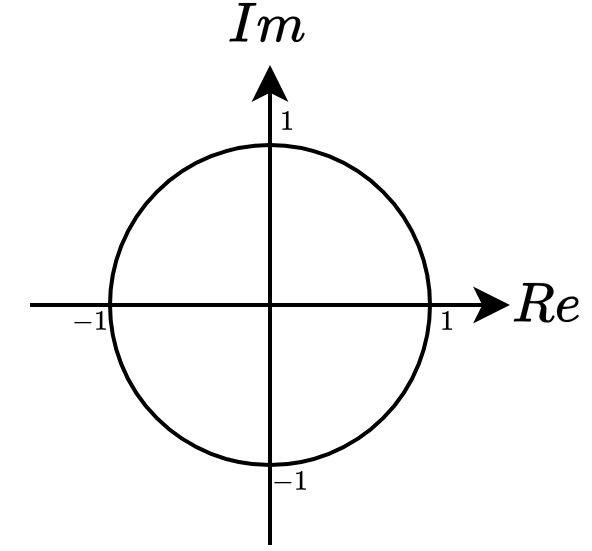
\includegraphics[width=0.3\linewidth]{images/unit.png}
    \caption{Unit circle in the complex plane}
\end{figure}
\begin{definition}[\textit{Minimum-phase transfer function}]
    If the zeros of $W(z)$ are also strictly inside the unit circle, $W(z)$ is termed minimum-phase.
\end{definition}

\paragraph*{Output stability}
\begin{theorem}
    The steady-state output $y(t)$ is stationary if and only if:
\end{theorem}
\begin{enumerate}
    \item \textit{$v(t)$ is stationary}. 
    \item \textit{$F(z)$ is asymptotically stable}. 
\end{enumerate}

\begin{theorem}
    There is only one stationary output corresponding to the steady-state solution.
    However, if $F(z)$ is asymptotically stable, then all potential outputs obtained for different initializations of the digital filter $F(z)$ converge asymptotically to the steady-state solution, i.e., to the stationary output.
\end{theorem}

\subsection{Models's transfer functions}
\paragraph*{Moving Average}
An MA($n$) process exhibits the following characteristics:
\begin{itemize}
    \item It possesses $n$ nontrivial zeros.
    \item It has $n$ poles, all located at the origin. 
\end{itemize}
This is a consequence of all Moving Average processes being generated by asymptotically stable filters.

\paragraph*{AutoRegressive}
An AR($m$) process is characterized by:
\begin{itemize}
    \item $m$ zeros, all positioned at the origin.
    \item $n$ nontrivial poles. 
\end{itemize}
Consequently, these processes are commonly referred to as all-poles processes.

\paragraph*{ARMA}
An ARMA($m,n$) process displays the following features:
\begin{itemize}
    \item $m$ nontrivial poles. 
    \item $n$ nontrivial zeros. 
\end{itemize}

It's noteworthy that if the input signal is a stationary stochastic process, and the transfer function leading to the output is asymptotically stable, then the resulting process is also a stochastic stationary one.